%!TEX root = main.tex
\section{Definitions and Conventions}
\label{sec:definitions}

This Section introduces definitions and conventions used through out this paper.
We define the undefinedness of an element $a \in A$ of a partial function $f$: $A \rightarrow B$ as
$f(a) = \bot$. We say $f[a \mapsto b]$ is the function $f'$ such that $f'(a) = b$ and
$f'(x) = f(x)$ otherwise. The same applies for all $a \in A'$ in $f[A' \mapsto b]$ where $A' \subseteq A$.
We define $f|_{A'}$ as the \textit{restriction} of $f$ to $A'$ as $f'$ such that
$f'(a) = f(a)$ if $a \in A'$, and $f'(a) = \bot$ for $a \not\in A'$. The inverse image
$\{ a \in A : f(a) = b\}$ for $b \in B$ will be written as $f^{-1}(b)$.


\begin{comment}
Introduces terms used in your topic by definitions. Furthermore, it 
can introduce theorems on which parts of your topic base. Hint: Use 
paragraphs to structure your text. This is the first paragraph.

And this is the second paragraph. By the way: Do not use 
abbreviations as don't, it's, or can't. In Figure~\ref{fig:graph} 
you can see an example of a picture embedded in a figure. The
picture is created using the TikZ-Library (cf. 
\href{../manuals/tikzpgfmanual.pdf}{TikZ-Manual}). In Table
\ref{tab:nameOfTheTable} you can see an example for a table.

\begin{definition}[Name of the term]
\label{def:nameOfTerm}
This is how you define a term.
\end{definition}

\begin{theorem}[Name of the theorem]
\label{the:nameOfTheorem}
This is how you write a theorem. Do not forget to prove the theorem.
\begin{proof}
	Here you write the proof of the theorem.
\end{proof}
\end{theorem}

\begin{figure}[htb] % where to insert the figure: h=here, t=top, b=bottom,
					% the order htb shows which position is preffered
	\begin{center}
		\begin{tabular}{cc}
			\begin{minipage}{0.35\linewidth} % minipages are a nice
											 % equipment to arrange
											 % pictures
				\begin{center}
					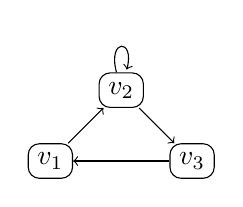
\begin{tikzpicture}[scale=0.9, 
				    state/.style={draw, rounded corners, fill=none,
				    			  text centered, text=black}]
	\node[state] (v1) at (0, 0) {$v_1$};
	\node[state] (v2) at (1, 1) {$v_2$};
	\node[state] (v3) at (2, 0) {$v_3$};
	\path[->] 	(v1)  edge 				node[] {} (v2)
				(v2)  edge[loop above] 	node[] {} (v2) 
				(v2)  edge 				node[] {} (v3)
				(v3)  edge 				node[] {} (v1);
\end{tikzpicture}

				\end{center}
			\end{minipage}
			&
			\begin{minipage}{0.55\linewidth} % note that the total
											 % width of the mini
											 % pages is less than
											 % 1.0\linewidth, since
											 % otherwise you get a
											 % badbox (try it yourself)
				\begin{center}
					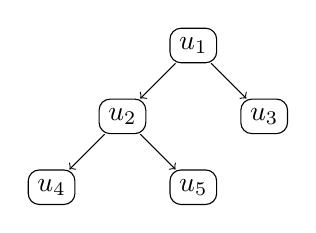
\begin{tikzpicture}[scale=0.9, 
				    state/.style={draw, rounded corners, fill=none,
				    			  text centered, text=black}]
	\node[state] (u1) at (7, 2) {$u_1$};
	\node[state] (u2) at (6, 1) {$u_2$};
	\node[state] (u3) at (8, 1) {$u_3$};
	\node[state] (u4) at (5, 0) {$u_4$};
	\node[state] (u5) at (7, 0) {$u_5$};
	\path[->] 	(u1)  edge   (u2);
	\path[->] 	(u1)  edge   (u3);
	\path[->] 	(u2)  edge   (u4);
	\path[->] 	(u2)  edge   (u5);
\end{tikzpicture}

				\end{center}
			\end{minipage}
		\end{tabular}
	\end{center}
	\caption{A digraph on the left and a directed tree on the right.}
	\label{fig:graph}
\end{figure}

In the next lines you can see some examples formulas and other
constructs, which are useful in the math mode. A very useful webpage
to find symbols and the packages to include is 
\href{http://detexify.kirelabs.org/classify.html}{Detexify$^2$}.
$\Sigma, \sigma, \ldots, \varphi, \xi$, \LaTeX
You can use the math mode in the text, e.g. $1\neq0$, or write it in
a whole line:
$$\left|
	\begin{array}{ccc}
		a_{1,1} & \ldots & a_{1,n}  \\
				& \vdots & 			\\
		a_{n,1} & \ldots & a_{n,n}
	\end{array}
\right|
\quad = \quad 
\left\{
	\begin{array}{ll}
			{\displaystyle \sum\limits_{\sigma\in S_n}} 
			% displaystyle avoids that symbols size get adjusted
			\left(
				\text{sgn}(\sigma)
				\prod\limits_{i=1}^{n}a_{i,\sigma(i)}
			\right) 
			& 
			\text{, if }True 
		\\[0.6cm] % adjust the line spacing
			{\displaystyle\frac{42}{1}} & \text{, otherwise}
	\end{array}
\right.$$


\begin{table}[htb]
	\caption{This a a table.}
	\label{tab:nameOfTheTable}
	\bigskip % Insert a vertical space. Also \smallskip or \medskip.
	\begin{center}
		\begin{tabular}{|l||l|c|r|}
			\hline
			& align left 	& centered & align right \\
			\hline \hline
			row $1$ & box $1.1$ & box $1.2$ & box $1.3$ \\
			\hline
			row $2$ & \multicolumn{2}{c|}{box $2.1$} & box $2.2$ \\
			\hline
			row $2$ & \multicolumn{3}{c|}{box $2$} \\
			\hline
		\end{tabular}
	\end{center}
\end{table}
\end{comment}